\subsubsection{Compara\c c\~ao dos Modelos}

Com o objetivo de obter uma análise mais aprofundada do desempenho de cada modelo, foi realizada uma comparação por meio de um gráfico de violino. Dessa forma, pôde-se observar qual dos modelos apresentava o melhor desempenho.



Ao examinar os modelos representados nas Figuras \ref{fig:modelos-arima} e \ref{fig:violin-lr-xgb-lgbm-rf}, identifico os modelos que se destacam em relação à natureza dos dados. Na Figura \ref{fig:basic_comparar}, que compara os modelos ARIMA e XGBoost com outros, torna-se evidente que os modelos ARIMA como AR, ARX, MA, ARMA, ARIMAX e SARIMAX demonstram um desempenho sólido. Além disso, os modelos baseados em gradientes e regressão, como o XGBoost, exibem resultados comparáveis, beneficiando-se da otimização por meio do Optuna, uma abordagem mais eficaz em relação aos tradicionais Grid Search e Randomized Search.

Na Figura \ref{fig:rrmse_comparar}, que contrasta as redes neurais com o modelo Prophet, é importante destacar que os modelos de redes neurais, incluindo RNN, LSTM, GRU, ANN, CNN e Transformer, foram avaliados em conjunto com o modelo Prophet. A análise estatística também demonstrou que o modelo RNN se sobressai como o vencedor entre as métricas avaliadas. Essa conclusão é respaldada pelas evidências de que pelo menos um modelo é superior aos demais. Os modelos com valores de p-valor abaixo de 0,05 foram realçados em \textit{itálico} para enfatizar sua significância.

A avaliação da eficácia dos modelos ARIMA em previsões de longo prazo emprega o teste de Ljung-Box, conforme detalhado no Apêndice \ref{sec:comtb18}. As Tabelas \ref{tb:lbtrn} a \ref{tb:lbcm} ilustram a acurácia dos modelos ARIMA ao longo do tempo, com valores menores sendo destacados em \textbf{negrito} e \textit{itálico} para facilitar a interpretação. Modelos como ARX, ARIMAX e SARIMAX, que incorporam variáveis exógenas, demonstram um desempenho superior nesse contexto. Esses modelos não lineares apresentam uma capacidade de previsão robusta em horizontes temporais mais longos, diferenciando-se positivamente dos outros modelos ARIMA.

\begin{figure}[H]
	\centering
	\caption{Comparação dos modelos ARIMA}\label{fig:modelos-arima}
	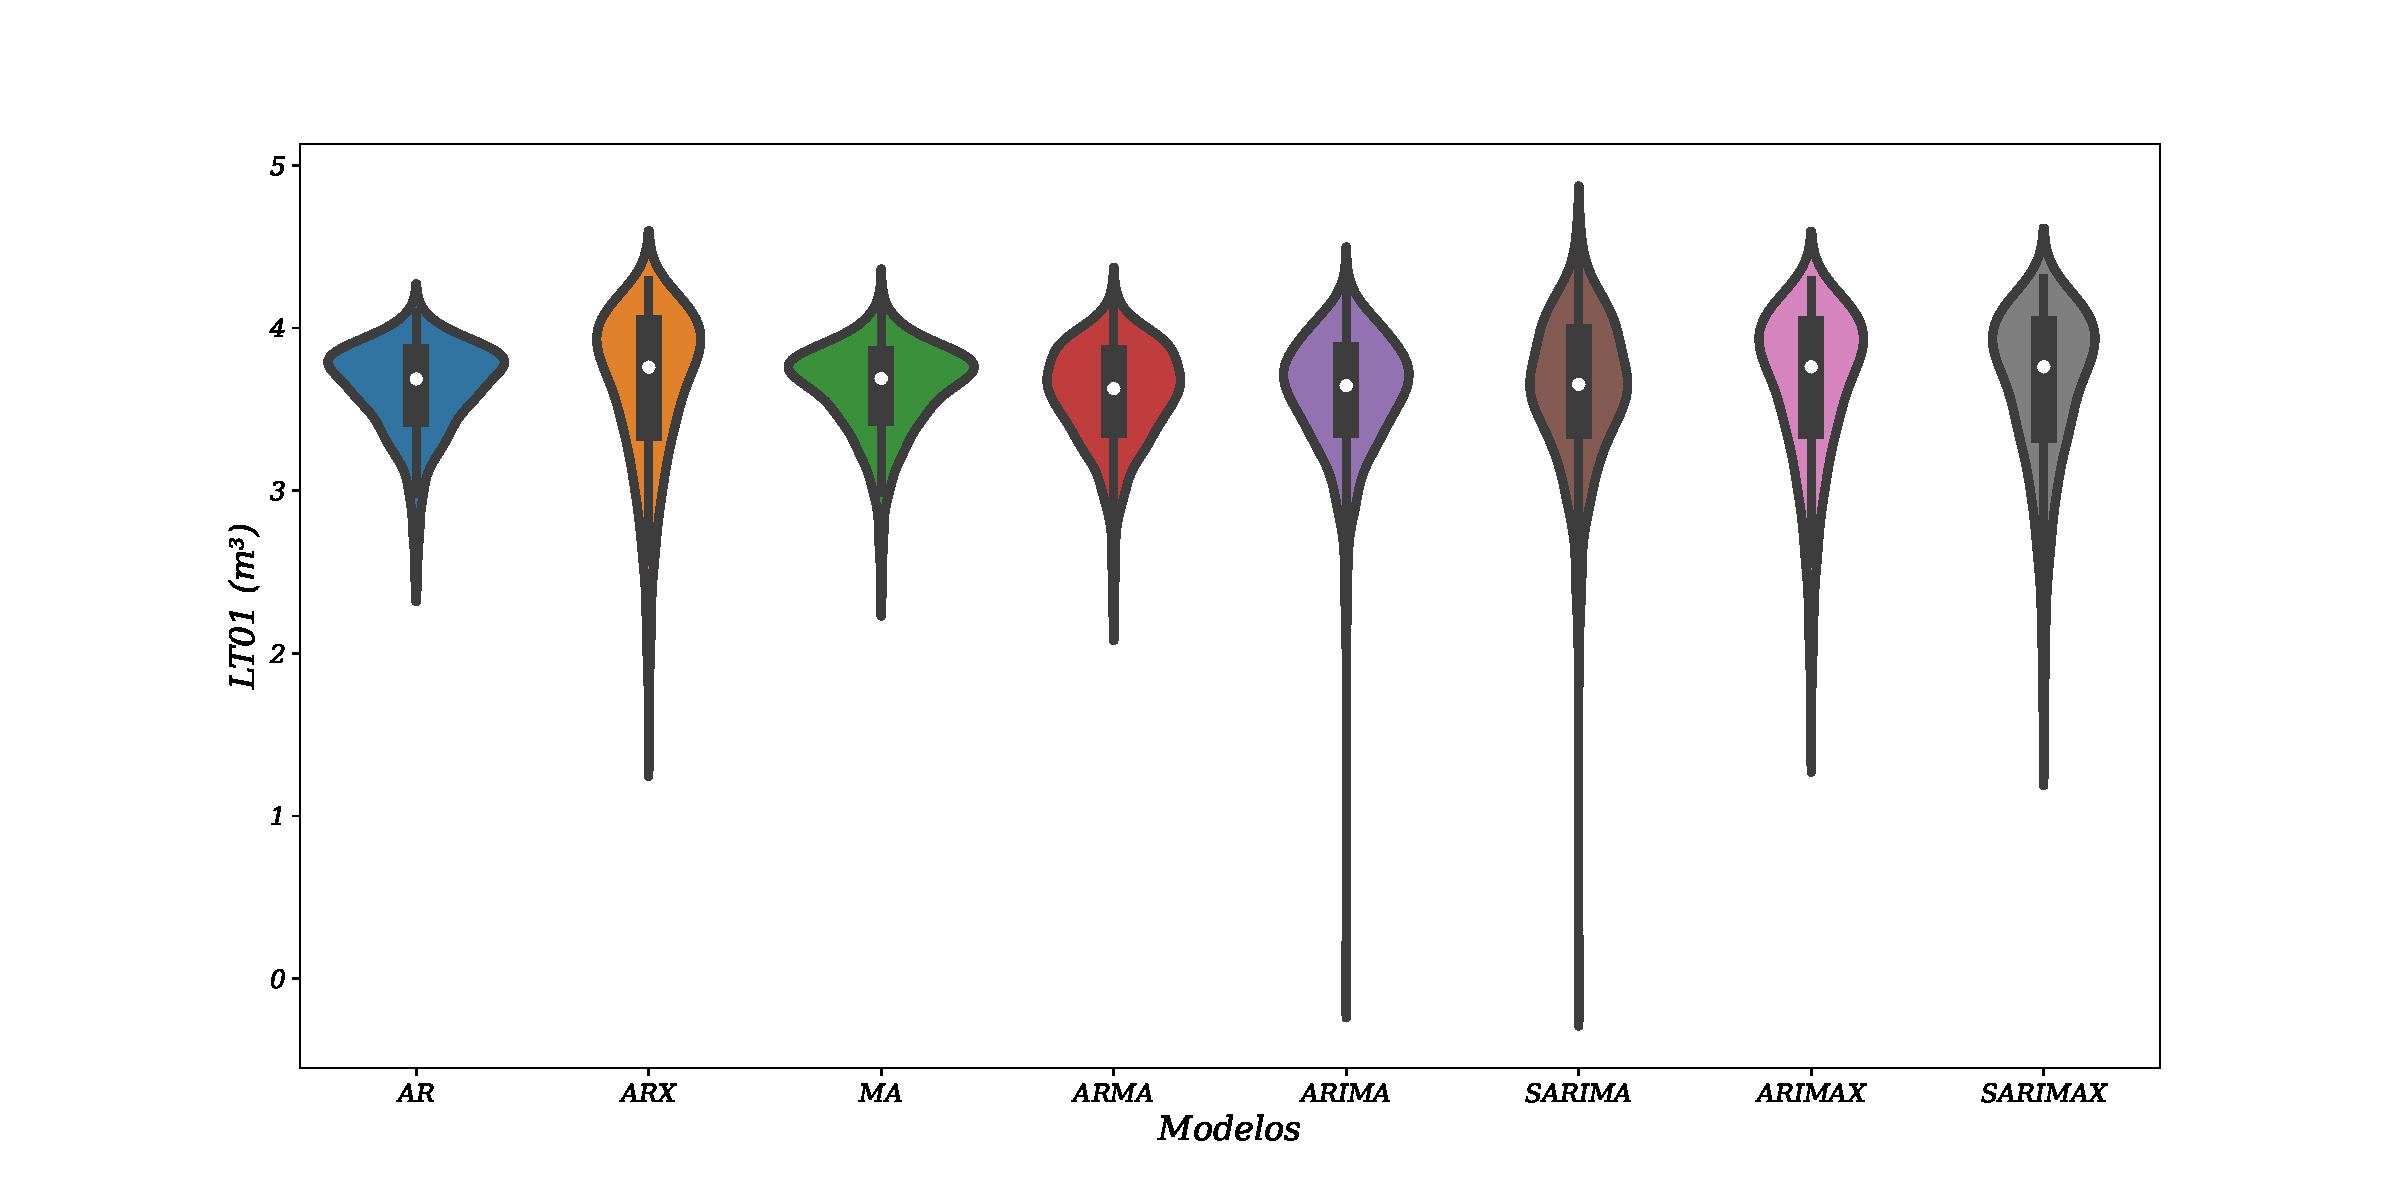
\includegraphics[width=0.8\linewidth]{Resultados/Figuras/modelos-arima}
	
	\fonte{Elaboração própria a partir de dados da SANEPAR (2018 a 2020)}
\end{figure}

\begin{figure}[!h]
	\centering
	\caption{Comparação de modelos de regressão}\label{fig:violin-lr-xgb-lgbm-rf}
	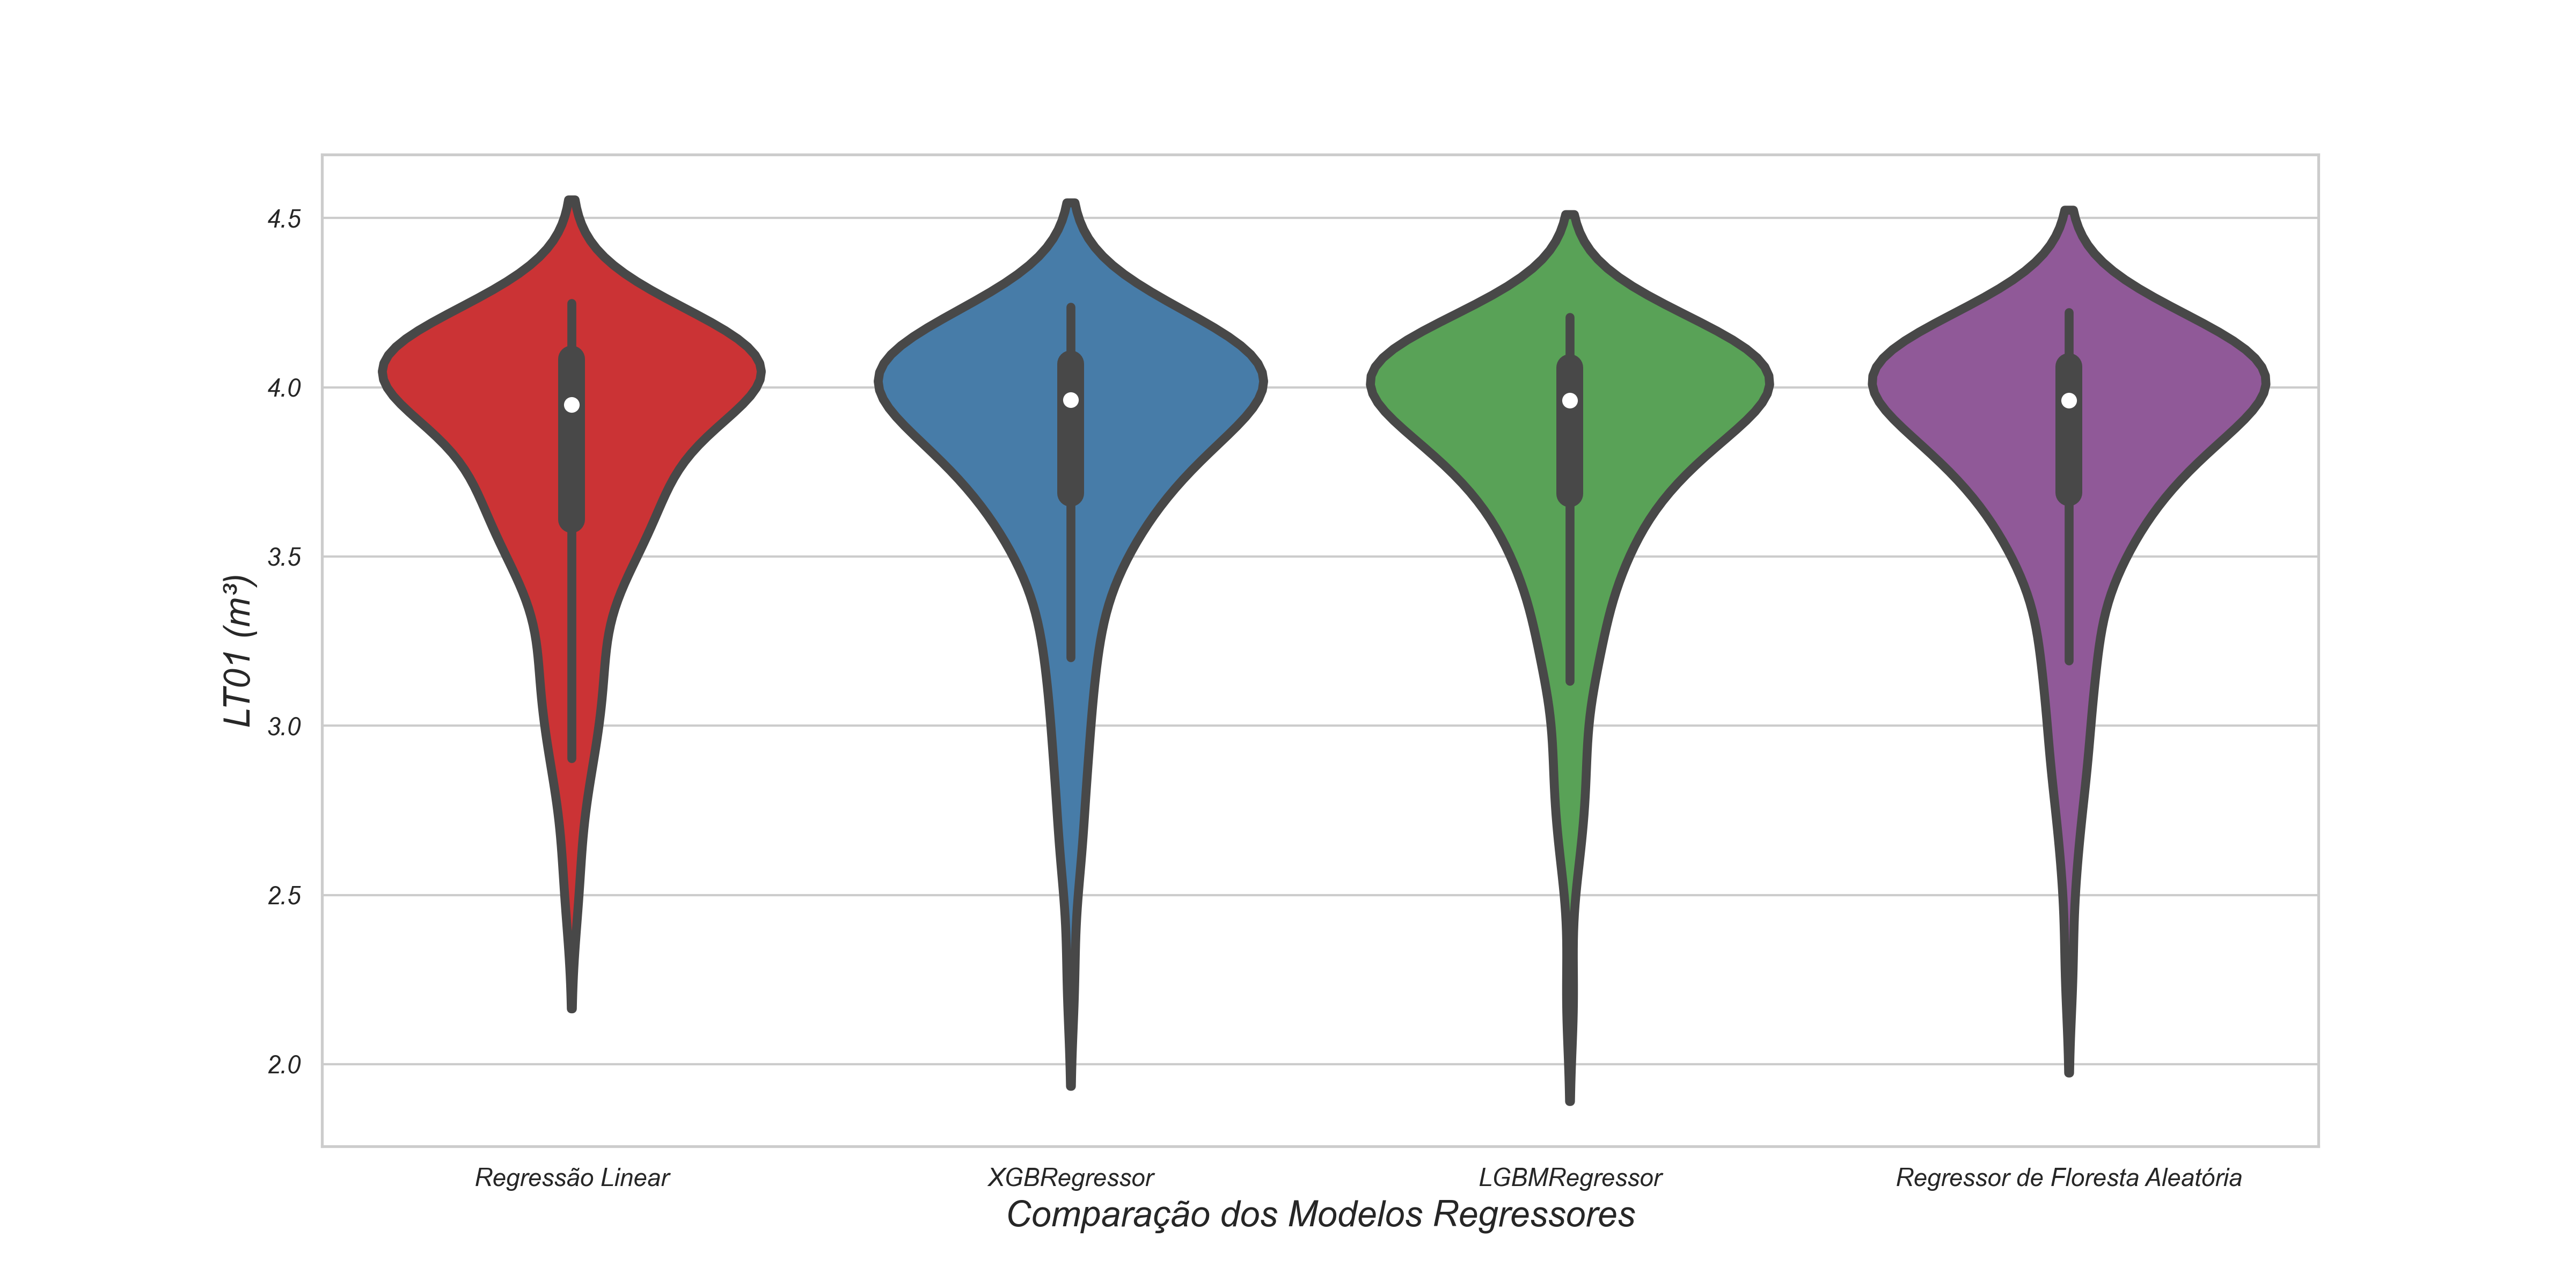
\includegraphics[width=0.8\linewidth]{Resultados/Figuras/violin-LR-XGB-LGBM-RF}
	
	
	
	\fonte{Elaboração própria a partir de dados da SANEPAR (2018 a 2020)}
\end{figure}

\begin{figure}[H]
	\centering
	\caption{Análise comparativa dos modelos utilizando gráfico de barras}
	\begin{subfigure}{0.8\textwidth}
		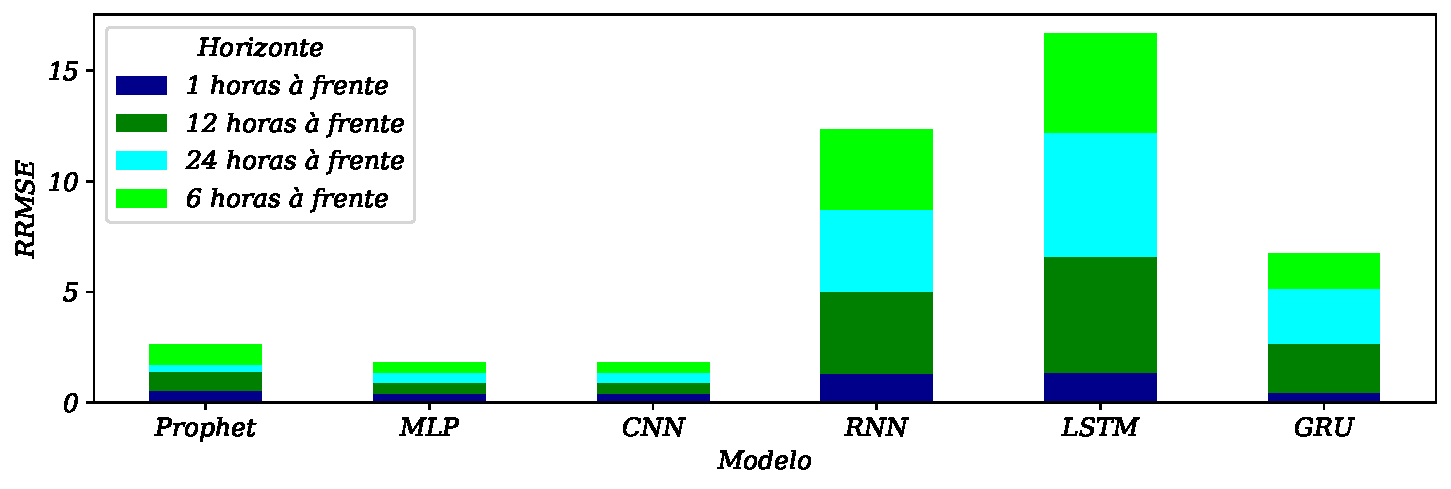
\includegraphics[width=\linewidth]{Resultados/Figuras/rrmse_comparar}
		\caption{Comparação de modelos de redes neurais e Prophet através da métrica RRMSE}
		\label{fig:rrmse_comparar}
	\end{subfigure}
	
	\begin{subfigure}{0.8\textwidth}
		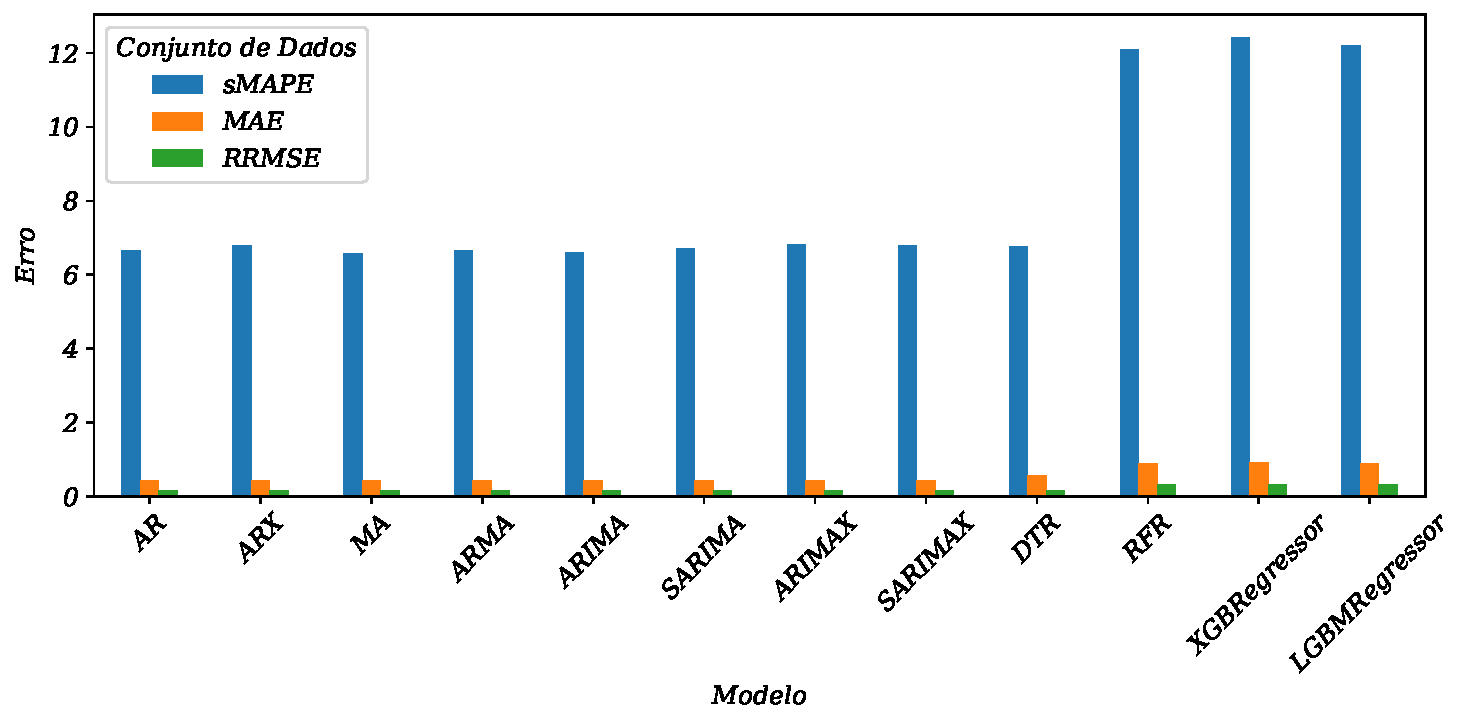
\includegraphics[width=\linewidth]{Resultados/Figuras/basic_comparar}
		\caption{Comparação de modelos}
		\label{fig:basic_comparar}
	\end{subfigure}
	
	\fonte{Elaboração própria a partir de dados da SANEPAR (2018 a 2020)}
\end{figure}

